
\documentclass{beamer}
\usepackage[latin1]{inputenc}
%\usetheme{Montpellier}
\usetheme{Boadilla}
%\usecolortheme[RGB={204,51,255}]{structure}
%\usecolortheme[named=purple]{structure}
\usecolortheme[RGB={62,128,62}]{structure}
%\definecolor{dark}{rgb}{0.3,0.15,0.3}
%\definecolor{light}{rgb}{0.8,0.6,0.8}
%\definecolor{reddish}{rgb}{.5,0.15,0.15}
\definecolor{dark}{rgb}{0.5,0.3,0.4}
%\definecolor{light}{rgb}{0.8,0.6,0.8}
\definecolor{reddish}{rgb}{.7,0.25,0.25}
\definecolor{greenish}{rgb}{.25,0.7,0.25}
\definecolor{blueish}{rgb}{.25,0.25,0.7}
\definecolor{purple}{rgb}{.5,0.0,0.5}
\usepackage{graphicx}
\usepackage{pstricks}

\usepackage{tikz}
\usetikzlibrary{arrows,decorations.markings,positioning}
\usepackage{epstopdf}

\title[9 The Gau\ss{}ian Distribution]{9 The Gau\ss{}ian Distribution}
\author{COMS10011}
\institute{\texttt{coms10011.github.io}}
\date{November 2019}

\begin{document}

\maketitle



\begin{frame}{Continuous random variables}
\color{black}
Continuous probability distributions work are defined
in terms of a density function \color{reddish}$p(x)$\color{black}:
\begin{itemize}
\item \color{reddish}$p(x)$\color{black} is like the probability per length
\end{itemize}
So to work out a probability for an interval
\color{reddish}
$$
\mbox{Prob}(x_1<x<x2)=\int_{x_1}^{x_2} p(x)dx
$$
\color{black}
\end{frame}

\begin{frame}{Introducing the Gau\ss{}ian distribution I}
\color{black}
\begin{itemize}
\item You can tell the Gau\ss{}ian distribution is important because it has different names: the \textsl{Gau\ss{}ian distribution}, the \textsl{normal distribution} or \textsl{the bell curve}.
\item It is a continuous distribution which is used to model a whole range of
natural phenomenon.
\item Much of statistics assumes almost everything has a Gau\ss{}ian distribution
\item There is a theorem we'll look at later, the \textsl{Central Limit Theorem}, that tells us why it is so common.
\end{itemize}
\end{frame}



\begin{frame}{Introducing the Gau\ss{}ian distribution II}
The Gaussian distribution
\color{purple}
$$
p(x)=\frac{1}{\sqrt{2\pi\sigma^2}}e^{-\frac{(x-\mu)^2}{2\sigma^2}}
$$
\color{black} where we'll show later that
\color{reddish}$\mu$\color{black}{} is the mean and
\color{reddish}$\sigma^2$\color{black}{}  is the variance, as you'd
expect from the choice of symbols.
\end{frame}

\begin{frame}{Introducing the Gau\ss{}ian distribution III}
The Gaussian distribution
\color{reddish}
$$
p(x)=\frac{1}{\sqrt{2\pi\sigma^2}}e^{-\frac{(x-\mu)^2}{2\sigma^2}}
$$
\color{black}
What about the \color{reddish}$1/\sqrt{2\pi\sigma^2}$\color{black}{}? That is there to normalize the curve:
\color{purple}
$$
\int_{-\infty}^\infty e^{-x^2/2\sigma^2}dx=\sqrt{2\pi\sigma^2}
$$
\color{black}
\begin{itemize}
\item We can do this particular definite integral
going from minus infinity to infinity, but the corresponding
indefinite integral can't be done.
\item There is a nice trick for doing the definite integral which we won't
  look at here for reasons of time.
\end{itemize}
\end{frame}

\begin{frame}{Introducing the Gau\ss{}ian distribution IV}
The Gaussian distribution for \color{reddish}$\mu=0$\color{black}{} and \color{reddish}$\sigma=1$\color{black}{}
\begin{center}
% GNUPLOT: LaTeX picture with Postscript
\begingroup
  \makeatletter
  \providecommand\color[2][]{%
    \GenericError{(gnuplot) \space\space\space\@spaces}{%
      Package color not loaded in conjunction with
      terminal option `colourtext'%
    }{See the gnuplot documentation for explanation.%
    }{Either use 'blacktext' in gnuplot or load the package
      color.sty in LaTeX.}%
    \renewcommand\color[2][]{}%
  }%
  \providecommand\includegraphics[2][]{%
    \GenericError{(gnuplot) \space\space\space\@spaces}{%
      Package graphicx or graphics not loaded%
    }{See the gnuplot documentation for explanation.%
    }{The gnuplot epslatex terminal needs graphicx.sty or graphics.sty.}%
    \renewcommand\includegraphics[2][]{}%
  }%
  \providecommand\rotatebox[2]{#2}%
  \@ifundefined{ifGPcolor}{%
    \newif\ifGPcolor
    \GPcolorfalse
  }{}%
  \@ifundefined{ifGPblacktext}{%
    \newif\ifGPblacktext
    \GPblacktexttrue
  }{}%
  % define a \g@addto@macro without @ in the name:
  \let\gplgaddtomacro\g@addto@macro
  % define empty templates for all commands taking text:
  \gdef\gplbacktext{}%
  \gdef\gplfronttext{}%
  \makeatother
  \ifGPblacktext
    % no textcolor at all
    \def\colorrgb#1{}%
    \def\colorgray#1{}%
  \else
    % gray or color?
    \ifGPcolor
      \def\colorrgb#1{\color[rgb]{#1}}%
      \def\colorgray#1{\color[gray]{#1}}%
      \expandafter\def\csname LTw\endcsname{\color{white}}%
      \expandafter\def\csname LTb\endcsname{\color{black}}%
      \expandafter\def\csname LTa\endcsname{\color{black}}%
      \expandafter\def\csname LT0\endcsname{\color[rgb]{1,0,0}}%
      \expandafter\def\csname LT1\endcsname{\color[rgb]{0,1,0}}%
      \expandafter\def\csname LT2\endcsname{\color[rgb]{0,0,1}}%
      \expandafter\def\csname LT3\endcsname{\color[rgb]{1,0,1}}%
      \expandafter\def\csname LT4\endcsname{\color[rgb]{0,1,1}}%
      \expandafter\def\csname LT5\endcsname{\color[rgb]{1,1,0}}%
      \expandafter\def\csname LT6\endcsname{\color[rgb]{0,0,0}}%
      \expandafter\def\csname LT7\endcsname{\color[rgb]{1,0.3,0}}%
      \expandafter\def\csname LT8\endcsname{\color[rgb]{0.5,0.5,0.5}}%
    \else
      % gray
      \def\colorrgb#1{\color{black}}%
      \def\colorgray#1{\color[gray]{#1}}%
      \expandafter\def\csname LTw\endcsname{\color{white}}%
      \expandafter\def\csname LTb\endcsname{\color{black}}%
      \expandafter\def\csname LTa\endcsname{\color{black}}%
      \expandafter\def\csname LT0\endcsname{\color{black}}%
      \expandafter\def\csname LT1\endcsname{\color{black}}%
      \expandafter\def\csname LT2\endcsname{\color{black}}%
      \expandafter\def\csname LT3\endcsname{\color{black}}%
      \expandafter\def\csname LT4\endcsname{\color{black}}%
      \expandafter\def\csname LT5\endcsname{\color{black}}%
      \expandafter\def\csname LT6\endcsname{\color{black}}%
      \expandafter\def\csname LT7\endcsname{\color{black}}%
      \expandafter\def\csname LT8\endcsname{\color{black}}%
    \fi
  \fi
  \setlength{\unitlength}{0.0500bp}%
  \begin{picture}(5040.00,3528.00)%
    \gplgaddtomacro\gplbacktext{%
      \csname LTb\endcsname%
      \put(858,440){\makebox(0,0)[r]{\strut{} 0}}%
      \put(858,793){\makebox(0,0)[r]{\strut{} 0.05}}%
      \put(858,1146){\makebox(0,0)[r]{\strut{} 0.1}}%
      \put(858,1499){\makebox(0,0)[r]{\strut{} 0.15}}%
      \put(858,1852){\makebox(0,0)[r]{\strut{} 0.2}}%
      \put(858,2204){\makebox(0,0)[r]{\strut{} 0.25}}%
      \put(858,2557){\makebox(0,0)[r]{\strut{} 0.3}}%
      \put(858,2910){\makebox(0,0)[r]{\strut{} 0.35}}%
      \put(858,3263){\makebox(0,0)[r]{\strut{} 0.4}}%
      \put(990,220){\makebox(0,0){\strut{}-4}}%
      \put(1447,220){\makebox(0,0){\strut{}-3}}%
      \put(1903,220){\makebox(0,0){\strut{}-2}}%
      \put(2360,220){\makebox(0,0){\strut{}-1}}%
      \put(2817,220){\makebox(0,0){\strut{} 0}}%
      \put(3273,220){\makebox(0,0){\strut{} 1}}%
      \put(3730,220){\makebox(0,0){\strut{} 2}}%
      \put(4186,220){\makebox(0,0){\strut{} 3}}%
      \put(4643,220){\makebox(0,0){\strut{} 4}}%
    }%
    \gplgaddtomacro\gplfronttext{%
    }%
    \gplbacktext
    \put(0,0){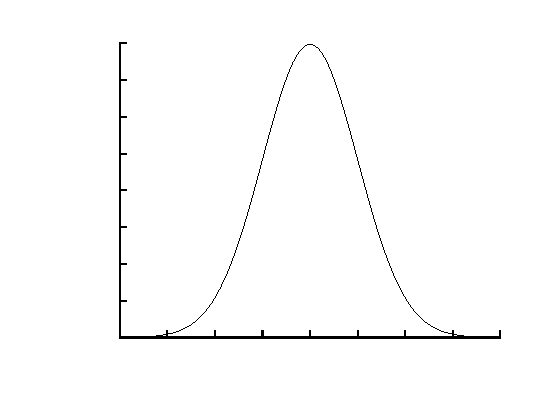
\includegraphics{fig_gauss}}%
    \gplfronttext
  \end{picture}%
\endgroup

\end{center}

\end{frame}


\begin{frame}{The moment generating function I}
Amazingly it is easier to work out the moment generating function than to work out the mean and variance directly. Recall
\color{reddish}
$$
m(t)=\langle e^{tX}\rangle
$$
\color{black}
and this allows you to work out the moments because
\color{reddish}
$$
\frac{d^nm}{dt^n}(0)=\mu_n
$$
\color{black}
where 
\color{reddish}
$$
\mu_n=\langle X^n\rangle
$$
\color{black}{}

\end{frame}



\begin{frame}{The moment generating function II}
So for the Gau\ss{}ian
\color{reddish}
$$
m(t)=\frac{1}{\sqrt{2\pi\sigma^2}}\int_{-\infty}^\infty \color{greenish}e^{xt}e^{-\frac{(x-\mu)^2}{2\sigma^2}}\color{reddish}dx
$$
\color{black}
Now using
\color{greenish}
$$
e^ae^b=e^{a+b}
$$
\color{black}
this gives 
\color{reddish}
$$
m(t)=\frac{1}{\sqrt{2\pi\sigma^2}}\int_{-\infty}^\infty \color{greenish}e^{-\frac{(x-\mu)^2}{2\sigma^2}+xt}\color{reddish}dx
$$

\end{frame}


\begin{frame}{The moment generating function III}
Now we have 
\color{reddish}
$$
m(t)=\frac{1}{\sqrt{2\pi\sigma^2}}\int_{-\infty}^\infty e^{\color{blueish}-\frac{(x-\mu)^2}{2\sigma^2}+xt\color{reddish}}dx
$$
\color{black}
and write
\color{blueish}{}
$$
\frac{(x-\mu)^2}{2\sigma^2}-xt=\frac{1}{2\sigma^2}(x^2-2\mu x +\mu^2-2\sigma^2 xt)
$$
\color{black}
then add and take away what is needed to make a square
\color{blueish}
\begin{eqnarray*}
x^2-2\mu x +\mu^2&-&2\sigma^2 xt\cr
 &=& x^2-2(\mu+\sigma^2 t) x +(\mu+\color{greenish}{}\sigma^2 t\color{blueish}{})^2\color{greenish}{} - 2\mu\sigma^2 t -\sigma^4 t^2\color{blueish}{}\cr
                                &=& (x-\mu-\sigma^2 t)^2 - 2\mu\sigma^2 t -\sigma^4 t^2
\end{eqnarray*}
\color{black}
\end{frame}


\begin{frame}{The moment generating function IV}

Hence
\color{reddish}
$$
m(t)=\frac{1}{\sqrt{2\pi\sigma^2}}\int_{-\infty}^\infty e^{-\frac{(x-\mu-\sigma^2 t)^2}{2\sigma^2}\color{greenish}{}+\mu t + \frac{1}{2}\sigma^2 t^2\color{reddish}}dx
$$
\color{black}
move the \color{greenish}{}stuff with no $x$s\color{black}{} outside the integral\color{reddish}
$$
m(t)=\left(\color{blueish}{}\frac{1}{\sqrt{2\pi\sigma^2}}\int_{-\infty}^\infty e^{-\frac{(x-\mu-\sigma^2 t)^2}{2\sigma^2}}dx\color{reddish}\right)\color{greenish}{} e^{\mu t + \frac{1}{2}\sigma^2 t^2}
$$
\color{black} and the \color{blueish}{}stuff in the big brackets\color{black}{} is just one,  it is the integral of the Gau\ss{}ian with mean \color{reddish}$\mu+\sigma^2 t$\color{black}{}, so
\color{purple}
$$
m(t)= e^{\mu t + \frac{1}{2}\sigma^2 t^2}
$$
\color{black}

\end{frame}

\begin{frame}{The mean and variance at last I}

Remember that 
\color{reddish}
$$
\frac{d^nm}{dt^n}(0)=\mu_n
$$
\color{black}
Now, rememember the chain rule
\color{greenish}{}
$$
\frac{d}{dt}e^{f(t)}=\frac{df}{dt}e^{f(t)}
$$
\color{black}
Using it we we get
\color{greenish}{}
$$
\frac{d}{dt}e^{\mu t + \frac{1}{2}\sigma^2 t^2}=(\mu+\sigma^2 t)e^{\mu t + \frac{1}{2}\sigma^2 t^2}
$$
\color{black}{}
If we set \color{reddish}$t=0$\color{black}{} this tells us that \color{reddish}$\langle X\rangle =\mu$\color{black}{}.


\end{frame}


\begin{frame}{The mean and variance at last II}

Going back to
\color{reddish}{}
$$
\frac{d}{dt}e^{\mu t + \frac{1}{2}\sigma^2 t^2}=(\mu+\sigma^2 t)e^{\mu t + \frac{1}{2}\sigma^2 t^2}
$$
\color{black}{}
we differenciate again to get
\color{reddish}
$$
\frac{d^2}{dt^2}e^{\mu t + \frac{1}{2}\sigma^2 t^2}=\frac{d}{dt}(\mu+\sigma^2 t)e^{\mu t + \frac{1}{2}\sigma^2 t^2}=[(\mu+\sigma^2 t)^2+\sigma^2]e^{\mu t + \frac{1}{2}\sigma^2 t^2}
$$
\color{black}{}
and if we set \color{reddish}$t=0$\color{black}{} we get \color{reddish}$\langle X^2\rangle =\sigma^2+\mu^2$\color{black}{} and
hence \color{reddish}$\langle X^2\rangle-\langle X\rangle^2=\sigma^2$\color{black}{}.

\end{frame}

\begin{frame}{Working out Gau\ss{}ian probabilities I}
\color{purple}
$$
\mbox{Prob}(x_1<x<x_2)=\frac{1}{\sqrt{2\pi\sigma^2}}\int_{x_1}^{x_2} e^{-\frac{(x-\mu)^2}{2\sigma^2}}dx
$$
\vskip -1cm
\color{black}
\begin{center}
% GNUPLOT: LaTeX picture with Postscript
\begingroup
  \makeatletter
  \providecommand\color[2][]{%
    \GenericError{(gnuplot) \space\space\space\@spaces}{%
      Package color not loaded in conjunction with
      terminal option `colourtext'%
    }{See the gnuplot documentation for explanation.%
    }{Either use 'blacktext' in gnuplot or load the package
      color.sty in LaTeX.}%
    \renewcommand\color[2][]{}%
  }%
  \providecommand\includegraphics[2][]{%
    \GenericError{(gnuplot) \space\space\space\@spaces}{%
      Package graphicx or graphics not loaded%
    }{See the gnuplot documentation for explanation.%
    }{The gnuplot epslatex terminal needs graphicx.sty or graphics.sty.}%
    \renewcommand\includegraphics[2][]{}%
  }%
  \providecommand\rotatebox[2]{#2}%
  \@ifundefined{ifGPcolor}{%
    \newif\ifGPcolor
    \GPcolorfalse
  }{}%
  \@ifundefined{ifGPblacktext}{%
    \newif\ifGPblacktext
    \GPblacktexttrue
  }{}%
  % define a \g@addto@macro without @ in the name:
  \let\gplgaddtomacro\g@addto@macro
  % define empty templates for all commands taking text:
  \gdef\gplbacktext{}%
  \gdef\gplfronttext{}%
  \makeatother
  \ifGPblacktext
    % no textcolor at all
    \def\colorrgb#1{}%
    \def\colorgray#1{}%
  \else
    % gray or color?
    \ifGPcolor
      \def\colorrgb#1{\color[rgb]{#1}}%
      \def\colorgray#1{\color[gray]{#1}}%
      \expandafter\def\csname LTw\endcsname{\color{white}}%
      \expandafter\def\csname LTb\endcsname{\color{black}}%
      \expandafter\def\csname LTa\endcsname{\color{black}}%
      \expandafter\def\csname LT0\endcsname{\color[rgb]{1,0,0}}%
      \expandafter\def\csname LT1\endcsname{\color[rgb]{0,1,0}}%
      \expandafter\def\csname LT2\endcsname{\color[rgb]{0,0,1}}%
      \expandafter\def\csname LT3\endcsname{\color[rgb]{1,0,1}}%
      \expandafter\def\csname LT4\endcsname{\color[rgb]{0,1,1}}%
      \expandafter\def\csname LT5\endcsname{\color[rgb]{1,1,0}}%
      \expandafter\def\csname LT6\endcsname{\color[rgb]{0,0,0}}%
      \expandafter\def\csname LT7\endcsname{\color[rgb]{1,0.3,0}}%
      \expandafter\def\csname LT8\endcsname{\color[rgb]{0.5,0.5,0.5}}%
    \else
      % gray
      \def\colorrgb#1{\color{black}}%
      \def\colorgray#1{\color[gray]{#1}}%
      \expandafter\def\csname LTw\endcsname{\color{white}}%
      \expandafter\def\csname LTb\endcsname{\color{black}}%
      \expandafter\def\csname LTa\endcsname{\color{black}}%
      \expandafter\def\csname LT0\endcsname{\color{black}}%
      \expandafter\def\csname LT1\endcsname{\color{black}}%
      \expandafter\def\csname LT2\endcsname{\color{black}}%
      \expandafter\def\csname LT3\endcsname{\color{black}}%
      \expandafter\def\csname LT4\endcsname{\color{black}}%
      \expandafter\def\csname LT5\endcsname{\color{black}}%
      \expandafter\def\csname LT6\endcsname{\color{black}}%
      \expandafter\def\csname LT7\endcsname{\color{black}}%
      \expandafter\def\csname LT8\endcsname{\color{black}}%
    \fi
  \fi
  \setlength{\unitlength}{0.0500bp}%
  \begin{picture}(5040.00,3528.00)%
    \gplgaddtomacro\gplbacktext{%
      \csname LTb\endcsname%
      \put(462,439){\makebox(0,0)[r]{\strut{} 0}}%
      \put(2619,220){\makebox(0,0){\strut{} $\mu$}}%
      \put(2872,220){\makebox(0,0){\strut{} $x_1$}}%
      \put(3479,220){\makebox(0,0){\strut{} $x_2$}}%
    }%
    \gplgaddtomacro\gplfronttext{%
    }%
    \gplbacktext
    \put(0,0){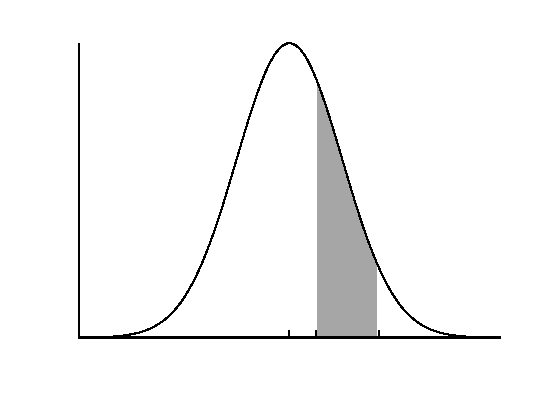
\includegraphics{fig_prob}}%
    \gplfronttext
  \end{picture}%
\endgroup

\end{center}
\end{frame}


\begin{frame}{Can't do the integral}
\color{reddish}
$$
\mbox{Prob}(x_1<x<x_2)=\frac{1}{\sqrt{2\pi\sigma^2}}\int_{x_1}^{x_2} e^{-\frac{(x-\mu)^2}{2\sigma^2}}dx
$$
\color{black}
The problem is we can't do this integral:
\begin{itemize}
\item We can't write this integral in terms of functions we know.
\item To get around this we define a new function specifically so we can relate the integral to that.
\item This is known as a \textsl{special function}, a new function defined for some special purpose.
\item The values of the special function can be calculated numerically.
\end{itemize}
\end{frame}


\begin{frame}{The error function}
\color{purple}
$$
\mbox{erf}\,(x)=\frac{1}{\sqrt{\pi}}\int_{-x}^xe^{-y^2}dy=\frac{2}{\sqrt{\pi}}\int_0^xe^{-y^2}dy
$$
\vskip -1cm
\color{black}
\begin{center}
% GNUPLOT: LaTeX picture with Postscript
\begingroup
  \makeatletter
  \providecommand\color[2][]{%
    \GenericError{(gnuplot) \space\space\space\@spaces}{%
      Package color not loaded in conjunction with
      terminal option `colourtext'%
    }{See the gnuplot documentation for explanation.%
    }{Either use 'blacktext' in gnuplot or load the package
      color.sty in LaTeX.}%
    \renewcommand\color[2][]{}%
  }%
  \providecommand\includegraphics[2][]{%
    \GenericError{(gnuplot) \space\space\space\@spaces}{%
      Package graphicx or graphics not loaded%
    }{See the gnuplot documentation for explanation.%
    }{The gnuplot epslatex terminal needs graphicx.sty or graphics.sty.}%
    \renewcommand\includegraphics[2][]{}%
  }%
  \providecommand\rotatebox[2]{#2}%
  \@ifundefined{ifGPcolor}{%
    \newif\ifGPcolor
    \GPcolorfalse
  }{}%
  \@ifundefined{ifGPblacktext}{%
    \newif\ifGPblacktext
    \GPblacktexttrue
  }{}%
  % define a \g@addto@macro without @ in the name:
  \let\gplgaddtomacro\g@addto@macro
  % define empty templates for all commands taking text:
  \gdef\gplbacktext{}%
  \gdef\gplfronttext{}%
  \makeatother
  \ifGPblacktext
    % no textcolor at all
    \def\colorrgb#1{}%
    \def\colorgray#1{}%
  \else
    % gray or color?
    \ifGPcolor
      \def\colorrgb#1{\color[rgb]{#1}}%
      \def\colorgray#1{\color[gray]{#1}}%
      \expandafter\def\csname LTw\endcsname{\color{white}}%
      \expandafter\def\csname LTb\endcsname{\color{black}}%
      \expandafter\def\csname LTa\endcsname{\color{black}}%
      \expandafter\def\csname LT0\endcsname{\color[rgb]{1,0,0}}%
      \expandafter\def\csname LT1\endcsname{\color[rgb]{0,1,0}}%
      \expandafter\def\csname LT2\endcsname{\color[rgb]{0,0,1}}%
      \expandafter\def\csname LT3\endcsname{\color[rgb]{1,0,1}}%
      \expandafter\def\csname LT4\endcsname{\color[rgb]{0,1,1}}%
      \expandafter\def\csname LT5\endcsname{\color[rgb]{1,1,0}}%
      \expandafter\def\csname LT6\endcsname{\color[rgb]{0,0,0}}%
      \expandafter\def\csname LT7\endcsname{\color[rgb]{1,0.3,0}}%
      \expandafter\def\csname LT8\endcsname{\color[rgb]{0.5,0.5,0.5}}%
    \else
      % gray
      \def\colorrgb#1{\color{black}}%
      \def\colorgray#1{\color[gray]{#1}}%
      \expandafter\def\csname LTw\endcsname{\color{white}}%
      \expandafter\def\csname LTb\endcsname{\color{black}}%
      \expandafter\def\csname LTa\endcsname{\color{black}}%
      \expandafter\def\csname LT0\endcsname{\color{black}}%
      \expandafter\def\csname LT1\endcsname{\color{black}}%
      \expandafter\def\csname LT2\endcsname{\color{black}}%
      \expandafter\def\csname LT3\endcsname{\color{black}}%
      \expandafter\def\csname LT4\endcsname{\color{black}}%
      \expandafter\def\csname LT5\endcsname{\color{black}}%
      \expandafter\def\csname LT6\endcsname{\color{black}}%
      \expandafter\def\csname LT7\endcsname{\color{black}}%
      \expandafter\def\csname LT8\endcsname{\color{black}}%
    \fi
  \fi
  \setlength{\unitlength}{0.0500bp}%
  \begin{picture}(5040.00,3528.00)%
    \gplgaddtomacro\gplbacktext{%
      \csname LTb\endcsname%
      \put(726,440){\makebox(0,0)[r]{\strut{}-1}}%
      \put(726,1146){\makebox(0,0)[r]{\strut{}-0.5}}%
      \put(726,1852){\makebox(0,0)[r]{\strut{} 0}}%
      \put(726,2557){\makebox(0,0)[r]{\strut{} 0.5}}%
      \put(726,3263){\makebox(0,0)[r]{\strut{} 1}}%
      \put(858,220){\makebox(0,0){\strut{}-4}}%
      \put(1331,220){\makebox(0,0){\strut{}-3}}%
      \put(1804,220){\makebox(0,0){\strut{}-2}}%
      \put(2277,220){\makebox(0,0){\strut{}-1}}%
      \put(2751,220){\makebox(0,0){\strut{} 0}}%
      \put(3224,220){\makebox(0,0){\strut{} 1}}%
      \put(3697,220){\makebox(0,0){\strut{} 2}}%
      \put(4170,220){\makebox(0,0){\strut{} 3}}%
      \put(4643,220){\makebox(0,0){\strut{} 4}}%
    }%
    \gplgaddtomacro\gplfronttext{%
    }%
    \gplbacktext
    \put(0,0){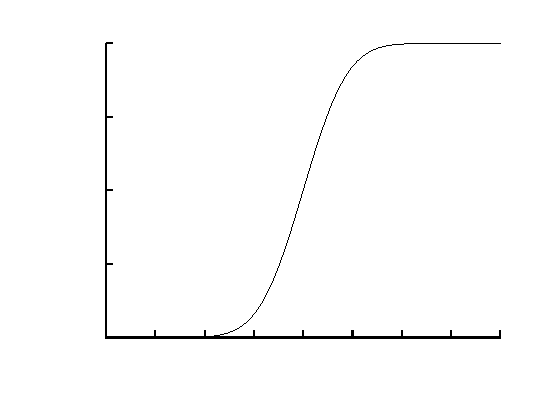
\includegraphics{fig_erf}}%
    \gplfronttext
  \end{picture}%
\endgroup

\end{center}
\end{frame}



\begin{frame}{Working out Gau\ss{}ian probabilities II}
So
\color{reddish}
$$
\mbox{Prob}(x_1<x<x_2)=\frac{1}{\sqrt{2\pi\sigma^2}}
\color{blueish}\int^{x_2}_{x_1}\color{reddish} 
e^{-\frac{(\color{blueish}{}x\color{reddish}-\mu)^2}{2\sigma^2}}\color{blueish}{}dx\color{reddish}
$$
\color{black}
Now do a change of variables
\color{blueish}{}
$$
z=\frac{x-\mu}{\sqrt{2}\sigma}
$$
\color{black}
so 
\color{blueish}{}
$$
dz=\frac{dx}{\sqrt{2}\sigma}
$$
\color{black}
and when \color{blueish}{}$x=x_1$\color{black}{} we have
\color{blueish}{}
$$
z=z_1=\frac{x_1-\mu}{\sqrt{2}\sigma}
$$
\color{black}
and for \color{blueish}{}$x=x_2$\color{black}{} similar.


\end{frame}

\begin{frame}{Working out Gau\ss{}ian probabilities III}
Putting this into the integral we have
\color{reddish}
$$
\mbox{Prob}(x_1<y<x_2)=\frac{1}{\sqrt{\pi}}\color{greenish}{}\int_{z_1}^{z_2}\color{reddish}{} e^{-\frac{z^2}{2}}dz
$$
\color{black}{}
then using
\color{reddish}
$$
\color{greenish}{}\int_a^b\color{reddish}f(x)dx=\color{greenish}{}-\int_b^a\color{reddish} f(x)dx
$$
\color{black}{}
and
\color{reddish}
$$
\color{greenish}{}\int_a^b\color{reddish}f(x)dx=\color{greenish}{}\int_a^0\color{reddish} f(x)dx+\color{greenish}{}\int_0^b\color{reddish} f(x)dx
$$
\color{black}{}
we have
\color{reddish}
$$
\mbox{Prob}(x_1<y<x_2)=-\frac{1}{\sqrt{\pi}}\color{greenish}{}\int_{0}^{z_1}\color{reddish}{} e^{-z^2}dz+\frac{1}{\sqrt{\pi}}\color{greenish}{}\int_{0}^{z_2}\color{reddish} e^{-z^2}dz
$$
\color{black}
\end{frame}

\begin{frame}{Working out Gau\ss{}ian probabilities IV}
Hence
\color{purple}
$$
\mbox{Prob}(x_1<x<x_2)=\frac{1}{2}[\mbox{erf}\,(z_2)-\mbox{erf}\,(z_1)]
$$
\color{black}{}
\end{frame}

\begin{frame}{An example}
\begin{itemize}
\item The loudness of songs at a concert are normally distributed with mean 75 dB and standard deviation\color{reddish}{} $\sigma=10 dB$\color{black}{}. 
\item What is the probability that the next song has loudness between 80 and 90 dB?
\end{itemize}
\color{reddish}
$$
\mbox{Prob}(80<x<90)=\frac{1}{2}[\mbox{erf}\,(\color{blueish}{}z_2\color{reddish})-\mbox{erf}\,(\color{blueish}{}z_1\color{reddish})]
$$
\color{black}
where 
\color{blueish}{}
$$
\sqrt{2}z_1=\frac{80-75}{10}=0.5
$$
\color{black}{}
and 
\color{blueish}{}
$$
\sqrt{2}z_2=\frac{90-75}{10}=1.5
$$
\color{black}{}
Working out numbers on a calculator or computer gives
\color{reddish}
$$
\mbox{Prob}(80<x<90)=0.2417
$$
\color{black}{}
\end{frame}



\end{document}

